\documentclass{pracamgr}
\usepackage{polski}
\usepackage[utf8]{inputenc}
\usepackage{amssymb}
\usepackage{amsmath}
\usepackage{amsthm}
\usepackage[pdftex]{graphicx}
\usepackage{multicol}
\usepackage{hyperref}

\author{Wiktor Zuba}

\nralbumu{320501}

\title{Efektywne algorytmy generacji obiektów kombinatorycznych???}

\tytulang{Effective algorithms of combinatorial objects generation???}

\kierunek{Informatyka}

\opiekun{prof. Wojciech Rytter\\
Instytut Informatyki}

\date{??? 2017}

\dziedzina{ 
 ???
}


\klasyfikacja{
???
}

\keywords{???}

\newtheorem{defi}{Definicja}[section]
\newtheorem{theorem}{Twierdzenie}
\newtheorem{lemma}[theorem]{Lemat}
\newtheorem{remark}[theorem]{Uwaga}
\newtheorem{corollary}[theorem]{Wniosek}


\begin{document}
\maketitle

\begin{abstract}
???
\end{abstract}


\tableofcontents%TODO podać, że overline coś to wektor, równy x_1,x_2,...,x_l plus może , overline0 to wektor z samych zer
%TODO wprowadzenie o funkcji Gamma i oszacowaniach na Gamma(k+1/2)/Gamma(k)

 \chapter*{Wprowadzenie}
 \addcontentsline{toc}{chapter}{Wprowadzenie}
  
 \chapter{Własności hiperkostki}
  \begin{defi}\label{hiperkostka}
   \emph{Hiperkostką wymiaru $n$ ($Q_n$)} nazwiemy graf, w którym każdy wierzchołek odpowiada ciągowi binarnemu długości $n$,
   zaś krawędzią połączone są te wierzchołki, których ciągi binarne różnią się na dokładnie jednej pozycji.\newline
   $V(Q_n)=\{(v_0,...,v_{n-1}):v_i\in\{0,1\}\}, E(Q_n)=\{(u,v):\sum_{i}|u_i-v_i|=1\}$
  \end{defi}
  \begin{center}
   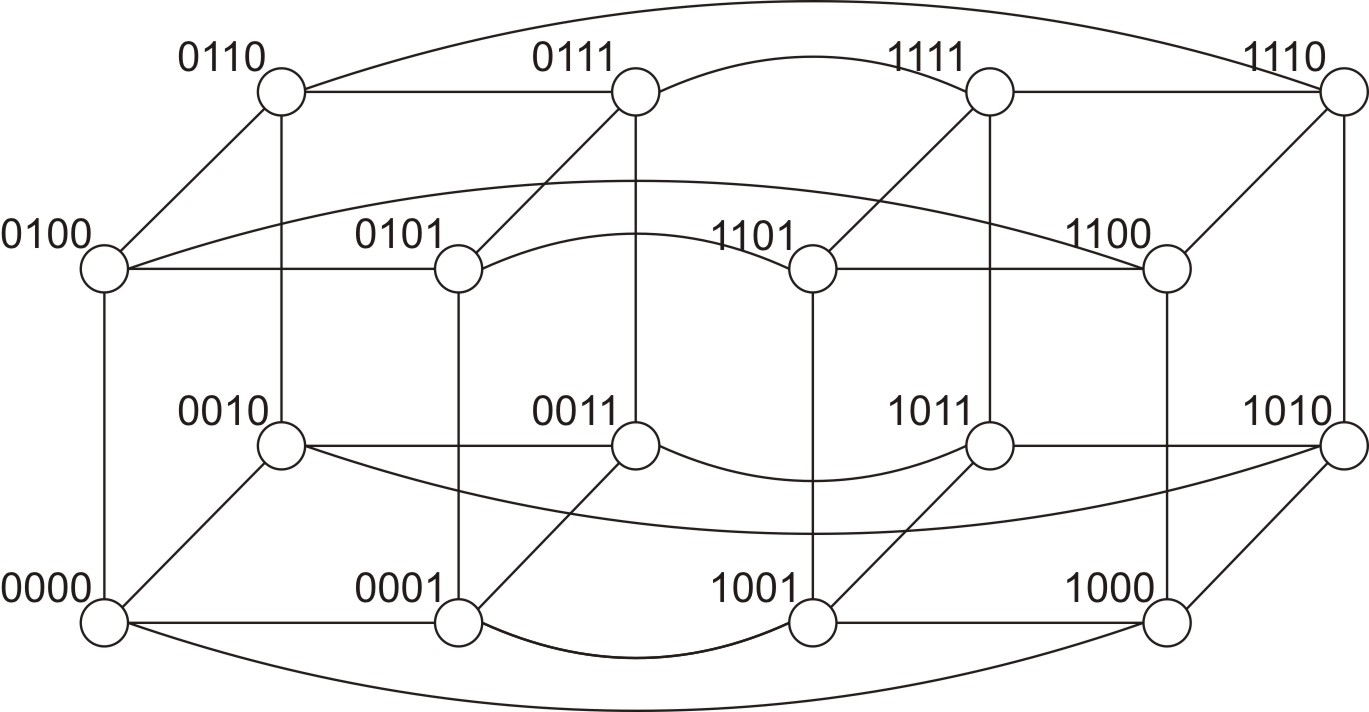
\includegraphics[scale=0.6]{Q_4.jpg}
  \end{center}
  W przypadku pełnej hiperkostki %TODO piszę o pełnej, więc trzeba dodać też że są te wadliwe
  bardzo łatwo jest określić długość najkrótszej ścieżki pomiedzy wierzchołkami --
  jest ona równa ilości pozycji na których róznią się ciągi tych wierzchołków.\newline
  Hiperkostka jest grafem dwudzielnym, w którym jedną składową jest zbiór wierzchołków o ciągach z parzystą liczbą jedynek,
  zaś drugą tych o ich nieparzystej liczbie.\newline
  Cowięcej przy badaniu hiperkostek często dzieli się je na $n+1$ warstw, gdzie dla $i\in\{0,1,...,n\}$ $i$-tą warstwę stanowią te wierzchołki,
  których ciągi binarne mają dokładnie $i$ jedynek (warstwa zawiera zatem wierzchołki oddalone o $i$ od wierzchołka zerowego ($\overline{0}$)).
  \begin{defi}\label{numerowanie klasyczne}
   \emph{Numerowaniem klasycznym (naturalnym)} hiperkostki nazwiemy takie numerowanie $\varphi:V(Q_n)\rightarrow\{1,...,|V(Q_n)|\}$ jej wierzchołków, że
   $\varphi(v)=1+\sum_{i}v_i\cdot2^i$
  \end{defi}
  \begin{center}
   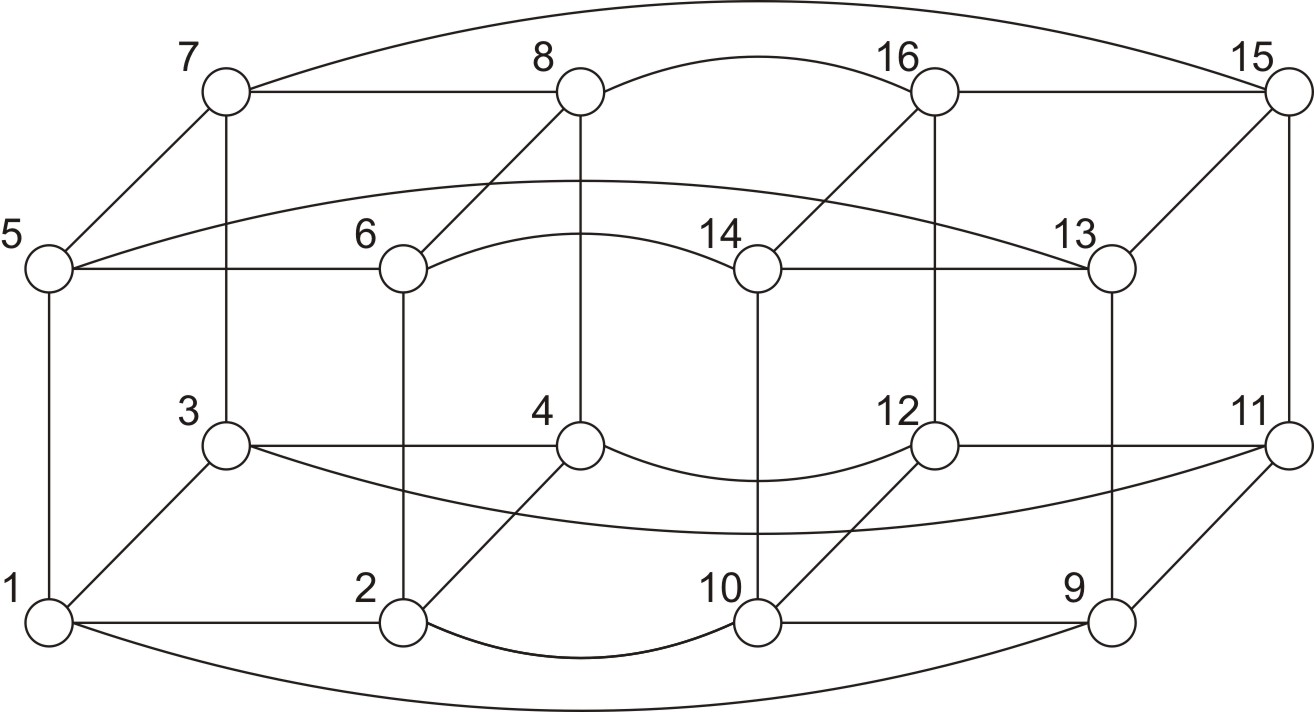
\includegraphics[scale=0.6]{Q_4(klasyczne).jpg}
  \end{center}
  \begin{defi}\label{numerowanie warstwowe}%TODO może n choose -1 nie jset tak bardzo standardowe
  \emph{Numerowaniem warstwowym} hiperkostki nazwiemy jej numerowanie w kolejności przeszukiwania grafu wszerz zaczynając od wierzchołka $\overline{0}$
  z wybieraniem sąsiadów w kolejności leksykograficznej.
  \end{defi}
  \begin{center}
   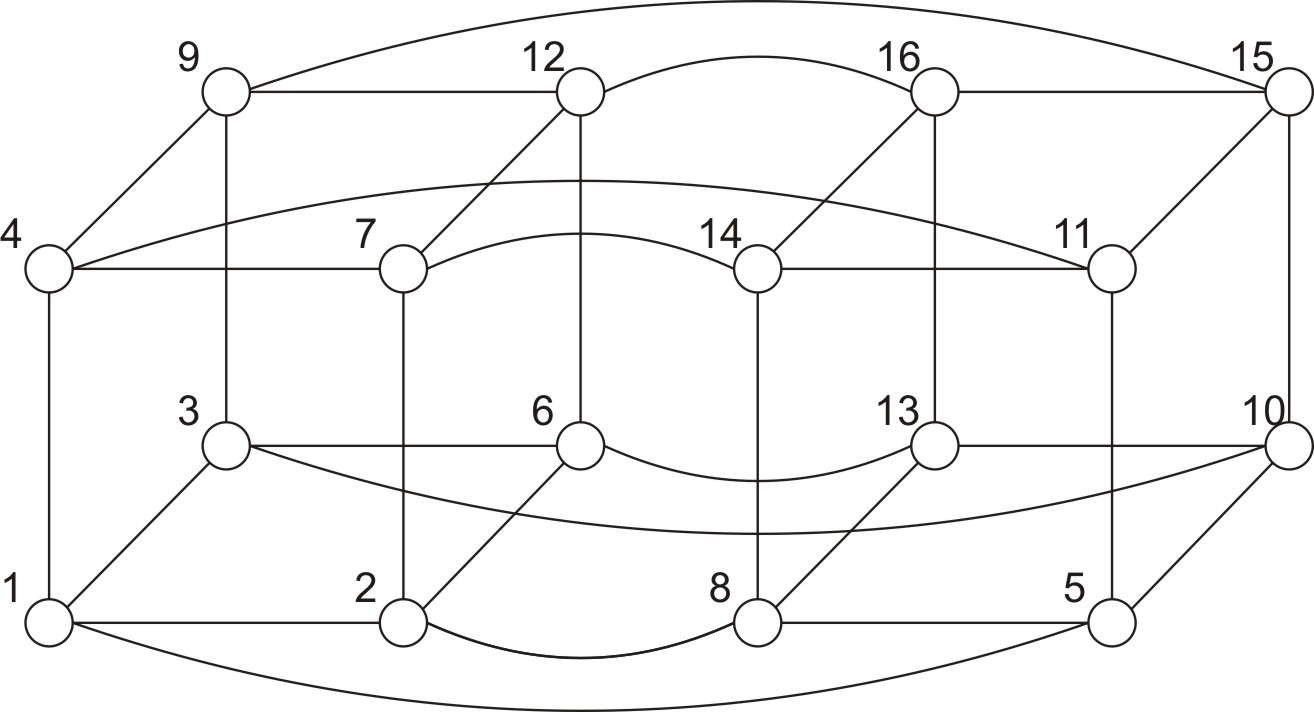
\includegraphics[scale=0.6]{Q_4(warstwowe).jpg}
  \end{center}   
  \begin{remark}\label{numerowanie warstwowe 2}
   Jest to takie numerowanie $\varphi:V(Q_n)\rightarrow\{1,...,|V(Q_n)|\}$ jej wierzchołków,
   że wierzchołki z $i$-tej warstwy otrzymują numery od $\sum_{j=0}^{i-1}{n\choose j}+1$ do $\sum_{j=0}^{i}{n\choose j}$.
   W obrębie jednej warstwy numery przyznawane są przeciwnie do kolejności leksykograficznej na odwróconych słowach.
   $\varphi(v)>\varphi(u)\Leftrightarrow (\sum_{i=0}^n v_i>\sum_{i=0}^n u_i)
   \vee((\sum_{i=0}^n v_i=\sum_{i=0}^n u_i)\wedge(\sum_{i=0}^n2^{n-i}v_i<\sum_{i=0}^n2^{n-i}u_i))$
  \end{remark}
  \begin{proof}
   Indukcyjnie po warstwach.\newline
   Dla warstwy $0$ oczywiste.\newline
   Zakładając, że $i$-ta warstwa jest ponumerowana w tym porządku weźmy dwa wierzchołki $u,v$ z warstwy $i+1$:
   $u=(\overline{y_1},1,\overline{x}),v=(\overline{y_2},0,\overline{x})$.\newline
   Jeśli $\overline{y_1}$ zawiera same $0$, to $\overline{y_2}$ zawiera dokładnie jedną $1$, sąsiedzi tych wierzchołków z poprzedniej warstwy
   o namniejszych numerach to odpowiednio $(\overline{0},0,x),(\overline{0},0,x)$,
   tak więc zostaną ponumerowane jako sąsiedzi tego samego wierzchołka, jednak $u$ otrzyma mniejszy numer jako sąsiad mniejszy leksykograficznie.\newline
   Jeśli $\overline{y_1}$ zawiera $1$, to $\overline{y_2}$ też, więc sąsiedzi tych wierzchołków z poprzedniej warstwy
   o namniejszych numerach to odpowiednio $(\overline{y'_1},1,\overline{x}),(\overline{y'_2},0,\overline{x})$, gdzie $\overline{y'_1}$ i $\overline{y'_2}$,
   to odpowiednio $\overline{y_1}$ i $\overline{y_2}$ z pierwszymi $1$ zamienionymi na $0$. Z założenia indukcyjnego sąsiad $u$ ma mniejszy numer niż sąsiad $v$,
   więc $u$ ma mniejszy numer niż $v$.
  \end{proof}
  \section{Podstawy kombinatoryczne}
   ${2n \choose n}=\frac{2^{2n}\Gamma(n+\frac{1}{2})}{\sqrt{\pi}\Gamma(n+1)}$\quad\quad
   ${2n+1 \choose n}={2n+1 \choose n+1}=\frac{2^{2n+1}\Gamma(n+\frac{3}{2})}{\sqrt{\pi}\Gamma(n+2)}$\newline
   $\Gamma(z)=\int\limits_{0}^{\infty}x^{z-1}e^{-x}dx$\quad
   dla $n\in\mathbb{N}$ $\Gamma(n)=(n-1)!$,\newline
   ogólniej dla $x\in\mathbb{R},x>1$ $\frac{\Gamma(x+1)}{\Gamma(x)}=x$,
   $\frac{\Gamma(x+\frac{1}{2})}{\Gamma(x)}<\frac{\Gamma(x+1)}{\Gamma(x+\frac{1}{2})}\Rightarrow
   \sqrt{x-\frac{1}{2}}<\frac{\Gamma(x+\frac{1}{2})}{\Gamma(x)}<\sqrt{x}$\newline
   \begin{lemma}\label{binomial sum upper bound}
    Dla $k<\lfloor\frac{n}{2}\rfloor$ zachodzi ograniczenie $\sum_{i=0}^{k-1}{n\choose i}<2^{n-1}\frac{{n\choose k}}{{n\choose \lfloor\frac{n}{2}\rfloor}}$
   \end{lemma}
   \begin{proof}
    (Uogólnienie dowodu z podobnego lematu dla n parzystych z \cite{LPV})\newline% Lemma3.8.2
    
   \end{proof}

  
  
  \section{Własność ekspansji}
  
   \begin{defi}\label{sasiedztwo wierzcholka}
    Dla grafu $G$ oraz wierzchołka $v\in V(G)$ definiujemy \emph{sąsiedztwo wierzchołka} jako zbiór wierzchołków połączonych z nim krawędzią:
    $N(v)=\{u\in V(G):(u,v)\in E(G)\}$.
   \end{defi}
   \begin{defi}\label{sasiedztwo zbioru wierzcholkow}%TODO może jakieś lepsze przetłumaczenie boundary
    Dla grafu $G$ oraz zbioru wierzchołków $S\subseteq V(G)$ definiujemy \emph{sąsiedztwo zbioru wierzchołków} jako zbiór tych sąsiadów wierzchołków ze zbioru,
    które same do tego zbioru nie należą: $N(S)=(\bigcup_{v\in S}N(v))\backslash S$
   \end{defi}
   \begin{defi}\label{wnetrze zbioru wierzcholkow}
    Dla grafu $G$ oraz zbioru wierzchołków $S\subseteq V(G)$ definiujemy \emph{wnętrze zbioru wierzchołków} jako zbiór tych wierzchołków z $S$,
    których wszyscy sąsiadzi również należą do tego zbioru: $In(S)=\{v\in S:N(v)\subseteq S\}$
   \end{defi}
   \begin{defi}\label{epsilon ekspansja wierzcholkowa}
    Graf $G$ posiada własność \emph{$\varepsilon$--ekspansji wierzchołkowej}, jeżeli dla każdego zbioru wierzchołków $S\subseteq V(G)$ takiego,
    że $|S|\le\frac{|V(G)|}{2}$ zachodzi $|N(S)|\ge\varepsilon\cdot|S|$
   \end{defi}
   \begin{lemma}
    Zbiór pierwszych $l$ wierzchołków hiperkostki według numerowania warstwowego posiada maksymalne wnętrze wśród zbiorów wielkości $l$.  
   \end{lemma}\label{HAR1}
   Jest to jeden z lematów dowodzonych w pracy \cite{HAR}.
   \begin{lemma}\label{S->S_k}%TODO chyba niezdefionowane S_k
    Dla hiperkostki do udowodnienia własności $\varepsilon_n$--ekspansji wierzchołkowej wystarczy rozważyć zbiory $S$ postaci $S_k,k\le 2^{n-1}$.
   \end{lemma}
   \begin{proof}
    Weżmy dowolne $S\subseteq V(G), l=|S|+|N(S)|$ z Lematu \ref{HAR1} wynika, że
    $\frac{|N(S)|}{|S|}=\frac{|N(S)|+|S|}{|S|}-1\ge\frac{|S_l|}{|In(S_l)|}-1=\frac{|S_l\backslash In(S_l)|}{|In(S_l)|}\ge\frac{|N(In(S_l))|}{|In(S_l)|}$.
    Z definicji $S_l$ wynika, że $In(S_l)=S_k$ dla $k=In(S_l)$.\newline
    Pozostaje udowodnić, że wystarczy rozważyć te $S_k$, że $k\le2^{n-1}$\newline
    Dla $l=|N(S)|+|S|\ge(\varepsilon_n+1)\cdot 2^{n-1}$ mamy $|S|>2^{n-1}$ lub $|N(S)|\ge\varepsilon_n|S|$, wystarczy więc rozważyć przypadek
    $l<(\varepsilon_n+1)\cdot 2^{n-1}$.\newline
    Dla $n=2m+1$ weżmy $k=2^{n-1}=\sum_{i=0}^{m}{2m+1 \choose i}$, wtedy $S_k$ = pełne $m+1$ pierwszych warstw i $N(S_k)$ = warstwa $m+1$.
    Przykład ten pokazuje, że $\varepsilon_n\le\frac{{2m+1 \choose m+1}}{2^{2m}}$,
    więc $l<2^{2m}+{2m+1 \choose m+1}\Rightarrow$ $S_l$ mieści się w piewszych $m+2$ warstwach
    $\Rightarrow$ $S_k=In(S_l)$ mieści się w pierwszych $m+1$ warstwach $\Rightarrow k\le 2^{2m}=2^{n-1}$.\newline
    Dla $n=2m$ weżmy $k=2^{n-1}=\sum_{i=0}^{m-1}{2m \choose i}+\frac{1}{2}{2m\choose m}$, wtedy $S_k$ = pełne $m$ pierwszych warstw + połowa środkowej.
    W środkowej warstwie pierwsze ${2m-1\choose m-1}=\frac{1}{2}{2m \choose m}$ wierzchołków to dokładnie te, których ciągi binarne kończą się na $1$.
    Wtedy też $S_k\cup N(S_k)$ to dokłanie pełne $m+1$ pierwszych warstw plus te wierzchołki z warstwy $m+2$, które kończą się na $1$
    $\Rightarrow |N(S_k)|={2m-1\choose m}+{2m-1\choose m}={2m-1\choose m-1}+{2m-1 \choose m}={2m\choose m}$.
    Przykład ten pokazuje, że $\varepsilon_n\le\frac{{2m \choose m}}{2^{2m-1}}$,
    więc $l<2^{2m-1}+{2m \choose m}\Rightarrow$ $S_l$ mieści się w piewszych $m+1$ warstwach plus tych wierzchołkach z warstwy $m+2$, które kończą się na $1$
    $\Rightarrow k\le2^{n-1}$.
   \end{proof}
   \begin{corollary}\label{ograniczenie ekspansji}
    Hiperkostka wymiaru $n$ nie posiada własności $\frac{2\sqrt{2}}{\sqrt{\pi n}}$--ekspansji wierzchołkowej.
   \end{corollary}
   \begin{proof}
    Dla $n=2m+1$\newline
    $\frac{|N(S_{2^{2m}})|}{|S_{2^{2m}}|}=\frac{{2m+1 \choose m+1}}{2^{2m}}=\frac{2\Gamma(m+\frac{3}{2})}{\sqrt{\pi}\Gamma(m+2)}<\frac{2}{\sqrt{\pi(m+1)}}=
    \frac{2}{\sqrt{\pi(\frac{n}{2}+\frac{1}{2})}}=\frac{2\sqrt{2}}{\sqrt{\pi(n+1)}}<\frac{2\sqrt{2}}{\sqrt{\pi n}}$.\newline
    Dla $n=2m$
    $\frac{|N(S_{2^{2m-1}})|}{|S_{2^{2m-1}}|}=\frac{{2m \choose m}}{2^{2m-1}}=\frac{2\Gamma(m+\frac{1}{2})}{\sqrt{\pi}\Gamma(m+1)}<\frac{2}{\sqrt{\pi m}}=
    \frac{2}{\sqrt{\pi\cdot\frac{n}{2}}}=\frac{2\sqrt{2}}{\sqrt{\pi n}}$.
   \end{proof}
   \begin{theorem}\label{ekspansja kostki}%TODO podać właściwe c
    Hiperkostka $Q_n$ posiada własność $\frac{c}{\sqrt{n}}$--ekspansji wierzchołkowej.
   \end{theorem}
   \begin{proof}
    Jeśli $k=\sum_{i=0}^{r}{n\choose i}$ (pełne $r$ warstw), to%TODO podać oszacowanie na sum {n\choose i}
    $\frac{|N(S_k)|}{|S_k|}=\frac{{n\choose r+1}}{\sum_{i=0}^{r}{n \choose i}}>\frac{{n\choose r+1}{n\choose \frac{n}{2}}}{2^{n-1}{n\choose r+1}}
    =\frac{{n\choose \frac{n}{2}}}{2^{n-1}}=\frac{2^n\Gamma(\frac{n}{2}+\frac{1}{2})}{2^{n-1}\sqrt{\pi}\Gamma(\frac{n}{2}+1)}=
    \frac{2\Gamma(\frac{n}{2}+\frac{1}{2})}{\sqrt{\pi}\Gamma(\frac{n}{2}+1)}>\frac{2}{\sqrt{\pi (\frac{n}{2}+\frac{1}{2})}}=
    \frac{2\sqrt{2}}{\sqrt{\pi (n+1)}}\ge\frac{2}{\sqrt{\pi n}}$.\newline

   \end{proof}


    


  
\begin{thebibliography}{99}%TODO dziwne czacionki
\addcontentsline{toc}{chapter}{Bibliografia}

  \bibitem{LPV} L. Lovasz, J. Pelikan and K. Vesztergombi.
   "Discrete Mathematics, Elementary and Beyond."
   \textit{Undergraduate Texts in Mathematics. New York: Springer, first edition, 2003}   


  \bibitem{HAR} L. H. HARPER,
   "Optimal Numberings and Isoperimetric Problems on Graphs"
   \textit{JOURNAL OF COMBINATORIAL THEORY 1, 385-393 (1966)}
   
   \bibitem{DFGKR} Tomas Dvorak, Jirı Fink, Petr Gregor, Vaclav Koubek and Tomasz Radzik,
   "Efficient connectivity testing of hypercubic networks with faults"
   
   
\end{thebibliography}

\end{document}